% Chapter 1
\chapter{Eaglescience [WIP]} % Chapter title

\label{ch:Eaglescience} % For referencing the chapter elsewhere, use \autoref{ch:introduction}

%----------------------------------------------------------------------------------------

Het hier beschreven onderzoek en daarbij behorende applicatie is geschreven in opdracht van Eaglescience wat gevestigd is in Amsterdam Sloterdijk. Eaglescience ontwikkeld complexe software op projectbasis voor diverse klanten vaak met een wetenschappelijke inslag. Het bedrijf telt +/- 20 medewerkers waarvan 75\% tot team eaglescience behoort en verantwoordelijk is voor de ontwikkeling van de geleverde software. de ander 25\% bekleed een support rol zoals project managers,  finance manager,  Quality manager etc. ). \\
Naast het ontwikkelen van nieuwe software biedt Eaglescience ook de mogelijkheid om zorg te dragen voor de eventuele hosting van het opgeleverde product. Hiermee kan Eaglescience nog beter garanderen dat de geboden kwaliteit in de software gewaarborgd blijft tijdens de levensduur van de software.

\section{Organisatie}
\marginpar{Organisatie}
Eaglescience bestaat uit drie divisies die elk onder Eaglescience B.V. vallen. Iedere divisie is verantwoordelijk voor een deel van die diensten die Eaglescience aanbied.
\begin{figure}[bth]
\myfloatalign
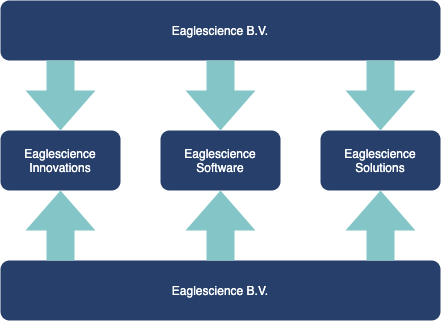
\includegraphics[width=10cm]{gfx/organogram}
\caption{Organogram Eaglescience}
\label{fig:Eaglescience organogram}
\end{figure}
% vragen Wat zijn de hoofddoelen van iedere divisie?
Eaglescience Innovations is op zoek naar nieuwe oplossingen op het gebied van software ontwikkeling en  die door de software tak wordt ge\"implementeert. Eaglescience Solutions is een divisie die samen met de klant opzoek gaat naar
een oplossing voor een gesteld probleem.
Het dagelijks bestuur is handen van:
\begin{itemize}
\item CEO - Marc Grootjen
\item CTO - Bas Breier
\item CFO - Wender van Mansvelt \\
\end{itemize}
Hieronder valt Team Eaglescience wat bestaat uit projectmanagers en ontwikkelaars
projectmanagers zijn verantwoordelijk voor het onderhoud met de klant over requirements en de bijbehorende bedrijfsmatige verstandhouding. De projectmanagers hebben de beschikking over een team ontwikkelaars die bestaan uit team Eaglescience. De ontwikkelaars zijn onderverdeeld onder de verschillende teams voor verschillende projecten. Op deze manier is een ontwikkelaar parallel betrokken bij meerdere projecten. Het kan dus voorkomen dat een ontwikkelaar op enig moment met meerdere projecten tegelijk bezig is wat de kennisdeling bevorderd.

\section{missie}
\marginpar{missie}
De missie van Eaglescience is het bedienen van onze partners door een ontwerp, ontwikkeling en service te bieden op het gebied van op maat gemaakte IT oplossingen . Om dit te kunnen bewerkstelligen heeft Eaglescience goed opgeleide IT professionals in dienst die zichzelf continue ontwikkelen op de “cutting edge” van IT technologie. De hoofd competenties van de medewerkers zijn: innovatief, intelligent, klant georientee\"erd, flexibel en ambitieus.

\section{visie}
Eaglescience streeft er als innovatief IT bedrijf naar om software te ontwikkelen als een Business-to-Business dienst. Met onze technische vaardigheden bouwen we veilige en hoogwaardige software die bijdraagt aan een betere wereld. Omdat we agile werken, leveren we precies wat nodig is, niets meer en niets minder. Wij helpen onze klanten zoeken naar een langdurige betrokkenheid en samenwerking op basis van zowel vertrouwen als wederzijds respect. \\
\marginpar{visie}
Omdat elke vraag uniek is, ontwikkeld Eaglescience op maar gemaakte en innovatieve software. We zijn van plan deel uit te maken van het hele proces van het formuleren van een idee tot het lanceren van het product en het waarborgen van de productie levenscyclus. Onze belangrijkste succesfactor zijn de mensen, die zich continu ontwikkelen door met de nieuwste technieken te werken op diverse projecten. Wij streven naar een optimale balans tussen werk en priv\'e. Dit geeft onze medewerkers veel vrijheid, maar vereist zelfdiscipline en verantwoordelijkheid.

\section{strategie}
Eaglescience levert de visie via vier strategische thema's:
\begin{itemize}
\item Maatschappelijke verantwoordelijkheid
\item Persoonlijke groei
\item Tevredenheid
\end{itemize}
\marginpar{strategische thema's}
We streven ernaar om veilige en hoogwaardige software diensten te leveren die waarde toevoegen aan onze samenleving. We streven naar een bedrijfscultuur waarin alle collega's hun talenten kunnen laten groeien. We hebben een ongecompliceerd werkethos: we richten ons op resultaten van hoge kwaliteit, maar met een gezonde balans tussen werk en priv\'e en voldoende tijd voor leuke en sociale evenementen. Eaglescience verwacht van alle medewerkers dat zij hun handelen baseren op vier kwaliteitsprincipes:
\begin{itemize}
\item Meld situaties die niet voldoen aan onze interne procedures
\item Evalueer risico's wanneer grote veranderingen worden verwacht
\item Help en daag elkaar uit
\item Kennis behouden over compliancy en kwaliteitsmanagement
\end{itemize}

\section{Werkwijze}
Zoals eerder gemeld werkt Eaglescience op projectbasis met ontwikkelaars in meedere teams. Er wordt getracht 'Full scrum" te werken waarbij de requirements van de klant centraal staan. Als een project wordt aangenomen door het management team dan wordt deze in sprints in samenwerking met de klant ontwikkeld. De klant wordt nauw betrokken bij het verloop van de ontwikkeling door middel van demo's aan het einde van iedere sprint, hier wordt gemeten hoe de applicatie zich gedraagt met betrekking tot de requirements van de klant. Dit is ook het moment dat er feedback gegeven wordt en waar waar nodig gestuurd kan worden in het verdere verloop. Op het moment dat er een applicatie klaar is wordt de software dan al niet overgedragen aan de klant of door gegeven aan support en hosting die verantwoordelijk zijn voor de daadwerkelijke hosting van de software.
\begin{figure}[bth]
\myfloatalign
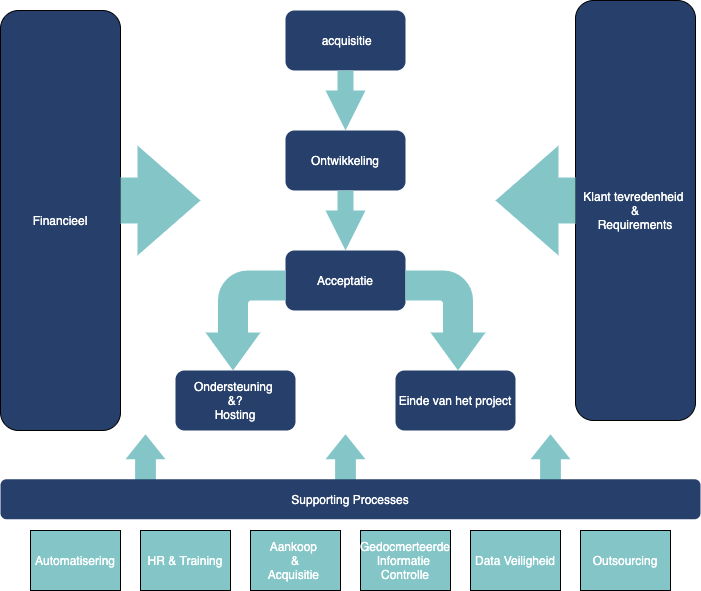
\includegraphics[width=10cm]{gfx/ProcessFlow}
\caption{Project Process}
\label{fig:Project Process}
\end{figure}
Naast het ontwikkel process zijn er een aantal supporting processes die ervoor zorgdragen dat het bedrijf blijft draaien en er nieuwe mensen aangenomen worden, maar ook een deel automatisering die voor ondersteuning zorgt voor platformen waarop ontwikkeld wordt.\\
Eaglescience ontwikkeld op projectbasis en op die manier komen er ook inkomsten. Dus alle processen die draaien moeten ingezet kunnen worden op projecten van klanten. Als er een project voor in huis gebruik wordt ondernomen moet er een duidelijk beeld zijn of er op termijn winst mee te behalen is op monetair vlak dan al niet tijdswinst of ontwikkel gemak.

\section{Relevante en actuele ontwikkelingen binnen Eaglescience}
Eaglescience is aan het groeien, zowel in het aantal projecten waar aan gewerkt wordt als het aantal medewerkers. Daarnaast worden de diensten die Eaglescience aanbied ook uitgebreid. Waarbij het hosten van de ontwikkelde applicaties steeds meer wordt aangeboden. Door deze inzet ligt de verantwoordelijk niet alleen bij het leveren van een veilige en hoogwaardige software maar het leveren van service waarbij de applicaties in een veilige omgeving worden aangeboden. Mede door de groei van het bedrijf maar zeker ook de diensten die aangeboden wordt is het zeer relevant om taken die geautomatiseerd kunnen worden te automatiseren.
